\documentclass[tikz,dvipdfmx,dvipsnames]{standalone}

\usepackage{amsmath, amssymb, amsthm, mathrsfs, amsfonts, dsfont}
\usepackage{bbm}
\usepackage{bm}
\usepackage{physics}
\usepackage{ifthen}
\usepackage{setspace}
\usepackage{mathtools}

\newcommand{\defeq}{\coloneqq}

\newcommand{\red}[1]{\textcolor{red}{#1}}
\newcommand{\blue}[1]{\textcolor{blue}{#1}}
\newcommand{\cyan}[1]{\textcolor{cyan}{#1}}
\newcommand{\gray}[1]{\textcolor{gray}{#1}}
\newcommand{\green}[1]{\textcolor{green}{#1}}
\newcommand{\brown}[1]{\textcolor{brown}{#1}}
\newcommand{\black}[1]{\textcolor{black}{#1}}
\newcommand{\orange}[1]{\textcolor{orange}{#1}}
\newcommand{\purple}[1]{\textcolor{purple}{#1}}
\newcommand{\yellow}[1]{\textcolor{yellow}{#1}}
\newcommand{\Magenta}[1]{\textcolor{Magenta}{#1}}
\newcommand{\RoyalBlue}[1]{\textcolor{RoyalBlue}{#1}}
\newcommand{\RubineRed}[1]{\textcolor{RubineRed}{#1}}
\newcommand{\ForestGreen}[1]{\textcolor{ForestGreen}{#1}}
\newcommand{\YellowOrange}[1]{\textcolor{YellowOrange}{#1}}
\newcommand{\WildStrawberry}[1]{\textcolor{WildStrawberry}{#1}}

\usetikzlibrary{calc,matrix,math}
\usetikzlibrary{decorations.pathreplacing,calligraphy}

\definecolor{c0}{RGB}{253, 231, 36}
\definecolor{c1}{RGB}{154, 216, 60}
\definecolor{c2}{RGB}{91, 200, 98}
\definecolor{c3}{RGB}{59, 81, 138}
\definecolor{c4}{RGB}{69, 50, 127}

\begin{document}

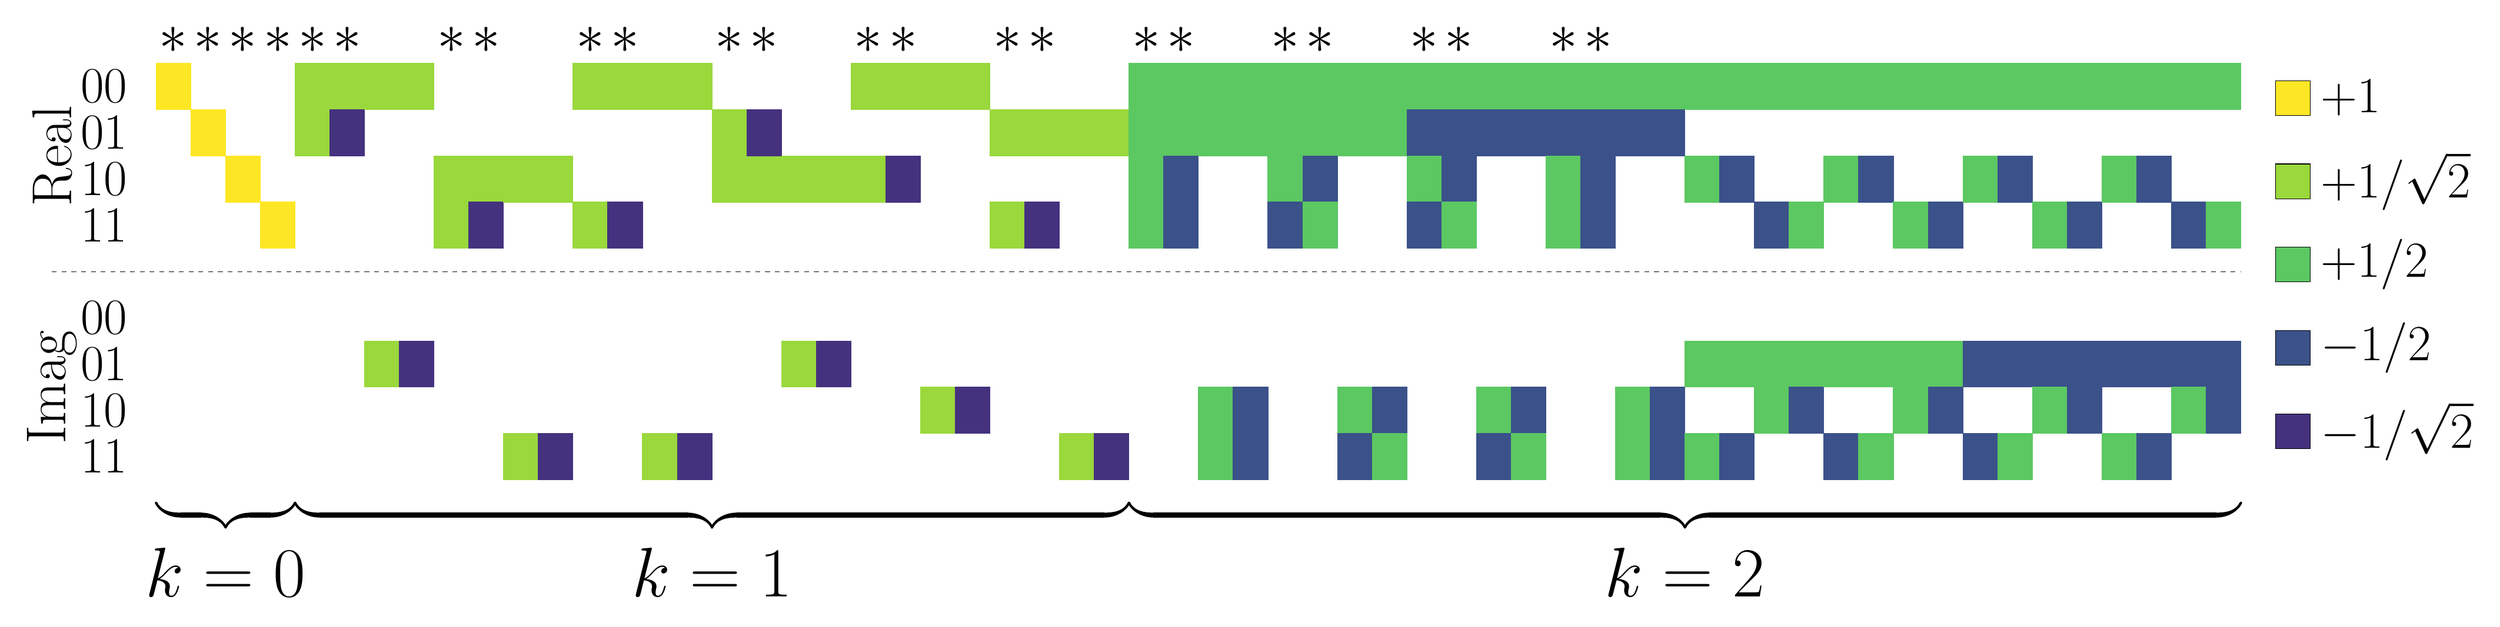
\begin{tikzpicture}[xscale=0.75]
    \foreach \color/\col/\row in {
            c0/0/0,
            c0/1/-1,
            c0/2/-2,
            c0/3/-3,
            c1/4/0,
            c1/4/-1,
            c1/5/0,
            c4/5/-1,
            c1/6/0,
            c1/6/-6,
            c1/7/0,
            c4/7/-6,
            c1/8/-2,
            c1/8/-3,
            c1/9/-2,
            c4/9/-3,
            c1/10/-2,
            c1/10/-8,
            c1/11/-2,
            c4/11/-8,
            c1/12/0,
            c1/12/-3,
            c1/13/0,
            c4/13/-3,
            c1/14/0,
            c1/14/-8,
            c1/15/0,
            c4/15/-8,
            c1/16/-2,
            c1/16/-1,
            c1/17/-2,
            c4/17/-1,
            c1/18/-2,
            c1/18/-6,
            c1/19/-2,
            c4/19/-6,
            c1/20/0,
            c1/20/-2,
            c1/21/0,
            c4/21/-2,
            c1/22/0,
            c1/22/-7,
            c1/23/0,
            c4/23/-7,
            c1/24/-1,
            c1/24/-3,
            c1/25/-1,
            c4/25/-3,
            c1/26/-1,
            c1/26/-8,
            c1/27/-1,
            c4/27/-8,
            c2/28/0,
            c2/28/-1,
            c2/28/-2,
            c2/28/-3,
            c2/29/0,
            c2/29/-1,
            c3/29/-2,
            c3/29/-3,
            c2/30/0,
            c2/30/-1,
            c2/30/-7,
            c2/30/-8,
            c2/31/0,
            c2/31/-1,
            c3/31/-7,
            c3/31/-8,
            c2/32/0,
            c2/32/-1,
            c2/32/-2,
            c3/32/-3,
            c2/33/0,
            c2/33/-1,
            c3/33/-2,
            c2/33/-3,
            c2/34/0,
            c2/34/-1,
            c2/34/-7,
            c3/34/-8,
            c2/35/0,
            c2/35/-1,
            c3/35/-7,
            c2/35/-8,
            c2/36/0,
            c3/36/-1,
            c2/36/-2,
            c3/36/-3,
            c2/37/0,
            c3/37/-1,
            c3/37/-2,
            c2/37/-3,
            c2/38/0,
            c3/38/-1,
            c2/38/-7,
            c3/38/-8,
            c2/39/0,
            c3/39/-1,
            c3/39/-7,
            c2/39/-8,
            c2/40/0,
            c3/40/-1,
            c2/40/-2,
            c2/40/-3,
            c2/41/0,
            c3/41/-1,
            c3/41/-2,
            c3/41/-3,
            c2/42/0,
            c3/42/-1,
            c2/42/-7,
            c2/42/-8,
            c2/43/0,
            c3/43/-1,
            c3/43/-7,
            c3/43/-8,
            c2/44/0,
            c2/44/-6,
            c2/44/-2,
            c2/44/-8,
            c2/45/0,
            c2/45/-6,
            c3/45/-2,
            c3/45/-8,
            c2/46/0,
            c2/46/-6,
            c2/46/-7,
            c3/46/-3,
            c2/47/0,
            c2/47/-6,
            c3/47/-7,
            c2/47/-3,
            c2/48/0,
            c2/48/-6,
            c2/48/-2,
            c3/48/-8,
            c2/49/0,
            c2/49/-6,
            c3/49/-2,
            c2/49/-8,
            c2/50/0,
            c2/50/-6,
            c2/50/-7,
            c2/50/-3,
            c2/51/0,
            c2/51/-6,
            c3/51/-7,
            c3/51/-3,
            c2/52/0,
            c3/52/-6,
            c2/52/-2,
            c3/52/-8,
            c2/53/0,
            c3/53/-6,
            c3/53/-2,
            c2/53/-8,
            c2/54/0,
            c3/54/-6,
            c2/54/-7,
            c2/54/-3,
            c2/55/0,
            c3/55/-6,
            c3/55/-7,
            c3/55/-3,
            c2/56/0,
            c3/56/-6,
            c2/56/-2,
            c2/56/-8,
            c2/57/0,
            c3/57/-6,
            c3/57/-2,
            c3/57/-8,
            c2/58/0,
            c3/58/-6,
            c2/58/-7,
            c3/58/-3,
            c2/59/0,
            c3/59/-6,
            c3/59/-7,
            c2/59/-3
        }{
            \draw[
                fill=\color,
                draw=\color
            ] (\col, \row) rectangle (\col + 1, \row - 1);
        }

    \foreach \row/\label in {
            -0.5/00,
            -1.5/01,
            -2.5/10,
            -3.5/11,
            -5.5/00,
            -6.5/01,
            -7.5/10,
            -8.5/11
        }{
            \node[anchor=center,font=\LARGE,scale=1.8]
            at (-1.5, \row) {\label};
        }

    \foreach \i in {
            0,1,2,3,4,5,8,9,12,13,16,17,20,21,24,25,28,29,32,33,36,37,40,41
        } {
            \node[anchor=center,font=\LARGE,scale=2] at (\i + 0.5, +0.5) {$*$};
        }

    \node[anchor=center,font=\LARGE,rotate=90,scale=2]
    at (-3, -2) {Real};
    \node[anchor=center,font=\LARGE,rotate=90,scale=2]
    at (-3, -7) {Imag};

    \draw[dashed] (-3,-4.5) -- (+60,-4.5);

    \foreach \l/\r/\k in {
            0/4/0,
            4/28/1,
            28/60/2
        }{
            \draw[decorate,
                decoration={calligraphic brace,mirror,amplitude=15pt},
                line width=3pt]
            (\l, -9.5) -- (\r, -9.5)
            node[
                midway, yshift=-1.5cm, font=\LARGE, scale=2.5
            ] {$k=\k$};
        }

    \begin{scope}[yscale=0.75,xshift=61cm]
        \draw[fill=c0] (0, 0.7-1*1.2) rectangle (1, 0.7-1*1.2-1);
        \draw[fill=c1] (0, 0.7-3*1.2) rectangle (1, 0.7-3*1.2-1);
        \draw[fill=c2] (0, 0.7-5*1.2) rectangle (1, 0.7-5*1.2-1);
        \draw[fill=c3] (0, 0.7-7*1.2) rectangle (1, 0.7-7*1.2-1);
        \draw[fill=c4] (0, 0.7-9*1.2) rectangle (1, 0.7-9*1.2-1);
        \node[anchor=west,font=\LARGE,scale=1.8] at (1, 0.7-1*1.2-0.5) {$+1$};
        \node[anchor=west,font=\LARGE,scale=1.8] at (1, 0.7-3*1.2-0.5) {$+1/\sqrt{2}$};
        \node[anchor=west,font=\LARGE,scale=1.8] at (1, 0.7-5*1.2-0.5) {$+1/2$};
        \node[anchor=west,font=\LARGE,scale=1.8] at (1, 0.7-7*1.2-0.5) {$-1/2$};
        \node[anchor=west,font=\LARGE,scale=1.8] at (1, 0.7-9*1.2-0.5) {$-1/\sqrt{2}$};
    \end{scope}
\end{tikzpicture}

\end{document}